\chapter{Corpus Preparation}
\label{chap:corpus}
Since this research is based on a supervised learning algorithm, a high-quality corpus is essential to our success. 

A expressive performance corpus is a set of performance samples. Each sample consists of a score and a recording. The score is the music notation being played, plus some metadata such as strucutre analusis, harmonic analysis etc.; the recording is a recording of a human musician playing the said score. A learning algorithm can learn how the music notation is transfromed into real performance. In this chapter, we will review the existing corpora, sample specifications and formats of a corpus, and how we construct the corpus used in this reasarch.

\section{Existing Corpora} 
Unlike research fields like speech processing or natural language processing, there exist very few public accessable corpus for research. CrestMusePEDB\cite{crestmuse} (PEDB stands for "Performance Expression Database"), created by Japan Science and Technology Agency's CREST program, is a rare example. It claims to contain the following data: PEDB-SCR - score text information, PEDB-DEV - performance deviation data and PEDB-IDX - audio performance credit. The database is said to be free to use via email request, but until the time this this writing, we can't establish any contact with the database andministrators, so the quality and format of the data is unknown.

Another example is the Magaloff Project\cite{magaloff}, which is a joint effort from a few universities in Austria.  Russian pianist Nikita Magaloff was invited to record all works for solo piano by Frederic Chopin on a Bösendorfer SE computer-controlled grand piano. This corpus became the material for many subsequent researches \cite{Goebl2009, Grachten2011, Flossmann2009, Grachten2012, Flossmann2013, Flossman2011, Flossmann2010a}. Flossmann et al., the leading researchers of the project, also won the 2008 RenCon contest with a expressive performance system call YQX\cite{yqx} based on this corpus. However, the corpus is not opened up in the public domain. 

\section{Corpus Specification}

Since we can't find any public corpus for our experiment, we need ot implement our own one. First, we need a clear specification of what will be included and will will not.

The corpus we need must fulfill the following constrains:
\begin{enumerate}
   \item All the samples are monophonic, containing only a single melody without chords.
   \item No human error, such as insertion, deletion, or wrong pitch exist in the recording; the score and recording are matched note-to-note.
   \item Phrasing information is given by human. 
   \item The score, recording and phrasing data are in machine-readable format.

   %\item The tempo label in MIDI recordings are the tempo by which the musician played. 
\end{enumerate}

There are many other useful information that can be included, but they are less relevant to our system, so they are not included. Examples are:

\begin{enumerate}
   \item Detailed Structural Analysis, such as GTTM (Generative Theory of Tonal Music)\cite{GTTM}
   \item Harmonic Analysis
   \item Musical Instrument specific instructions, such as violin pizzicato, tapping, or bow techniques.
   \item Musical Instrument specific instructions, such as piano fingering, violin bow techniques etc.
   \item Piano paddle usage
\end{enumerate}

Clementi's Sonatina Op. 36 is chosen as the repertoire of the corpus.  Because  Clementi's Sonatina is a basic repertoire almost every piano student in Asia will learn, so it' s easy to find performers with different skill level to record the corpus. Clementi wrote these sonatinas in classical style, so the skill required to play them can be easily extended to other classical era works like Mozart or Haydn. This fact makes the learned model a very general one, which is good for evaluation. There are six sonatinas included in Op. 36, the first five have three movements each, and the last one has two movements. The titles, tempo markers and time signautres of all the pieces in Op. 36 are listed in Table \ref{tab:cleminfo}

\begin{table}
   \centering
   \caption{Clementi's Sonatinas Op. 36 }
   \label{tab:cleminfo}
   \begin{tabular}{lll}
      \hline
      \textbf{Title} & \textbf{Movement} & \textbf{Time Signature}\\
      \hline
      No. 1 Sonatina in C major&    I. Allegro &4/4\\
      &    II. Andante &3/4\\
      &    III. Vivace &3/8\\
      No. 2 Sonatina in G major&    I. Allegretto &2/4\\
      &    II. Allegretto &3/4\\
      &    III. Allegro &3/8\\
      No. 3 Sonatina in C major&    I. Spiritoso &4/4\\
      &    II. Un poco adagio &2/2\\
      &    III. Allegro &2/4\\
      No. 4 Sonatina in F major&    I. Con spirito &3/4\\
      &    II. Andante con espressione &2/4\\
      &    III. Rondó: Allegro vivace &2/4\\
      No. 5 Sonatina in G major&    I. Presto &2/2\\
      &    II. Allegretto moderato &3/8\\
      &    III. Rondó: Allegro molto &2/4\\
      No. 6 Sonatina in D major&    I. Allegro con spirito &4/4\\
      &    I. Allegro con spirito &6/8\\
      \hline
   \end{tabular}
\end{table}


There are many digital format for score to choose from, such as MusicXML\cite{Good2001}, LilyPond\cite{LilyPond}, Finale, Sibelius, ABC, MuseData, and Humdrum. The book \cite{Selfridge-Field1997} has a comprehensive review on this issue. %For research purpose, proprietary format like Finale and Sibelius is abandoned because of their limited support from open source tools. 
We choose MusicXML as our score format. MusicXML is a score notation system using XML (eXtensible Markup Language) representation, it can express most music notations and metadata, and its specification is publicly available, so most music notation software and computer music code library will support musicXML format. An example snippet of a musicXML score is shown in Fig. \ref{fig:expxml}%LilyPond is a \LaTeX-like language for music typesetting. %ABC, MuseData and Humdrum are based on ASCII codes and each defines their unique representation for music score. 
\begin{figure*}[tp]
   \begin{center}
      %TODO:Fig.:Example JSON code
      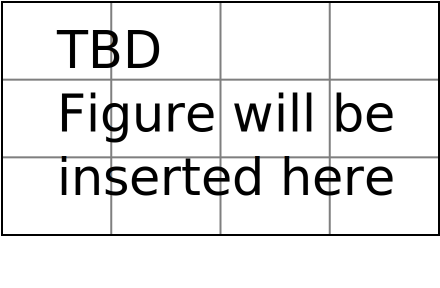
\includegraphics[width=\textwidth]{fig/TBDFigure}

   \end{center}
   \caption{Example MusicXML score}
   \label{fig:expxml}
\end{figure*}
%TODO: guitar pro?
Although MIDI is also a popular candidate for score representation in computer music research, it is designed to hold instrument control signal rather than notation. Some printed music notations may not be available in MIDI.  Furthermore, MIDI represents music as a series of note on and off events, which in nature does not fit the mental model of traditional music notation system.

But for performance, MIDI is the most suitable format.
Although an WAV (Waveform Audio Format) audio recording has higher fidelity than MIDI, it takes extra effort to annotate the notes, either manually or automatically. Since onset detection and pitch detection algorithms still can't achieve perfect accuracy, manually labeling is inevitable, which will soon become an impossible if manpower is not sufficient. On the other hand, a MIDI recording can provide exact timing, key pressure, and pitch for each note, even in polyphonic recordings. 

There's one possible way to keep the score and recording in one single MIDI file. Instead of recording the exact note on and note off timing, the nominal note on and off time are kept on the beats, which is exactly the same on the score. Then, MIDI tempo-change events are inserted before each note to represent the real timing of the recorded notes. This way we can merge the two files into one. But since MIDI is a limited medium for score, as discussed in early section, and it requires complex calculations to recover the performance from fixed notes and tempo-change events, this method is not used in the research.
%A human musician can't play every note exactly on the beat, even if playing along with a metronome. There are two ways to record this behavior: first, record the exact note-on and note-off time, while keeping the tempo fixed; second, keep the notes on the beat, so the MIDI looks the same as the score. Then insert tempo-change event between each notes, so notes of the same length can be rendered differently because they have different tempo marker. The second method may look smart, because the score and performance can be stored in one MIDI file instead of two, but it would involve complex calculation when linearly scaling the tempo. Since tempos from different samples need to be normalized during feature extraction, the first method is superior  than the second.
%Other formats such as image files (scanned or typesetted by computer) or PDF files are an alternative, but they are not an option for direct computer analysis. 

%In this research, we use MusicXML as the main vehicle for music score, because of the following reasons: first, it covers most music notations and metadata need for this research. Second, it is supported in most music notation software, including the one used in this research -- MuseScore. Finally, the music21 toolbox can convert many other formats into MusicXML without problem.

Finally, metadata not in the score and performance need to be stored somewhere. The only metadata we used is the phrasing. We store the phrasing in a plaintext file, each line in the phrasing file is the starting point of each phrase. The starting point is defined as the onset timing (in quarter notes) from the starting of the piece\footnote{For a phrase that start at a point which is a circulating decimal, the starting point can be defined as any finite decimal between the end of the last phrase and the start of the current phrase. For example, if the last phrase stops at beat 1, the second phrase start at $2\frac{1/3}=2.333\cdots$ beat, the start point of the second phrase can be written as 2.3 or 2.0, etc.} The phrasing is assigned by the author, but since phrasing controls the structural expression of a piece, anyone can create their own phrasing file to make the system learn their phrasing decision.  For our corpus, the boundaries of phrases are defined by the following features:
\begin{enumerate}
   \item Salient pause.
   \item Cadence
   \item Dramatic change in tempo, key or loudness
   \item Repeated structures in tempo or pitch.
\end{enumerate}
The above are just general principles, not strict rules, the phrasing is still decided by subjective analysis.




 
%\section{File Format}
\section{Implementation}

\subsection{Score Preparation}

The digital score used is downloaded from KernScore website \cite{KernScores}. The original format is in Hundrum file format (.krn), they are transformed into MusicXML by music21 toolkit. Because this research focus on monophonic melody only, the accompaniments are remove and the chords are reduced to their highest pitched note, which is usually the most salient melody line. Since the accompaniment removal and chord reduction process is done by automated scripts, the bugs in the related musicXML parser will introduce errors. So the output is compared to a printed version publish by Durand \& Cie.,Paris \cite{Clementi1915} to eliminate any error. We use MuseScore notation editor to view and edit MusicXML; some metadata errors are corrected by editing the MusicXML with text editors .

\subsection{MIDI Recording}
We have implemented two methods to record an expressive performance: First, using a Yamaha digital piano to record MIDI. Second, by tapping on a laptop computer touchpad to express tempo, duration and loudness. Due to data accuracy consideration, only recordings from Yamaha digital piano are selected.


To record the MIDI performances, we used a Yamaha P80 88-key graded hammer effect\footnote{Graded Hammer Effect feature provides realistic key pressure response similar to a traditional acoustic piano}digital piano. The Yamaha keyboard was connected to a MIDI-to-USB  converter so it acted as a USB MIDI device on a Linux computer. On the Linux computer we use Rosegarden Digital Audio Workstation (DAW) to record MIDIs. The Rosegarden DAW also generated the metronome sound to help the performer maintain a steady speed. One may argue that the tempo variation is also a part of the expression, but if the performer plays freely, the tempo information written in the MIDI file will be invalid, which makes subsequent parsing and manipulation a very hard task. So the performers are asked to follow the speed of the metronome, but they can apply any level of rubato they like. 

\framebox{TODO: touch pad recordings}
The second method, which is not used in the final experiments, is utilizing the Synaptics Touchpad on a Lenovo X200i laptop. When the user tap the touchpad, one note from the score will be played and recorded, when the user taps again, the next note will be played. The timing and pressure of the tapping event will be translated to the note's onset, duration and loudness. This idea have already be used in musical toys\cite{toyviolin} and musical games. If this input mechanism is turned into a game, we can easily collect large quantity of training input from laptops and smartphones with touchscreen. But the problem with this method is the lack of accuracy in pressure, because the touchpad use the touched surface area to estimate the pressure. So we did not use samples from this method, but in early experiments we did find this method a plausible alternative to MIDI keyboard.

\subsection{MIDI Cleaning and Phrase Splitting}
  After the MIDIs are recorded, a utility script is employed to check each recording is matched note-to-note with its corresponding score; if not, the mistakes are manually corrected using MIDI editing software. For example, if the pitch was played wrongly, we will correct the pitch but keep the onset, duration  and intensity as is. If there their are small segements that are beyond simple fix, repeated or similar segments from the same piece are used as a reference to reconstruct the wrongly-performed segment. The matched score and MIDI pair are then splat into phrases according to the corresponding phrasing file using a script. The splitted phrases are checked again for note-to-note match to avoid bugs in the scripts.

\section{Results}

Clementi's Sonatina Op. 36 has six pieces, the number of phrases (accorduing to our phrasing) and notes are shown in Table \ref{tab:clemcount}. The length distibution of the phrases in six pieces are shown in Fig. \ref{fig:phrlength}
\framebox{TODO: distribution of corpus}
Six graduate students (not majored in music) with a varying piano skill. Their piano-related experiences are shown in Table \ref{tab:performer}. Five of them finished Clementi's entire Op. 36, the last one only recorded part of the work. The total number of recordings and the corresponding phrases/notes counts are shown in Table \ref{tab:corpuscount}. 

\framebox{BOOKMARK}

\begin{table}[bp]
   \centering
   \caption{Phrases and Notes Count for Clementi's Sonatina Op. 36}
   \label{tab:clemcount}
   \begin{tabular}{lrr}
      \hline
      \textbf{Title}&\textbf{Phrases Count}&\textbf{Notes Count}\\
      \hline
      No. 1 Mov. I&12&222\\
      No. 1 Mov. II&10&147\\
      No. 1 Mov. III&16&261\\
      No. 2 Mov. I&18&320\\
      No. 2 Mov. II&6&125\\
      No. 2 Mov. III&28&414\\
      No. 3 Mov. I&25&526\\
      No. 3 Mov. II&6&74\\
      No. 3 Mov. III&19&438\\
      No. 4 Mov. I&25&465\\
      No. 4 Mov. II&12&222\\
      No. 4 Mov. III&16&384\\
      No. 5 Mov. I&17&672\\
      No. 5 Mov. II&13&316\\
      No. 5 Mov. III&24&564\\
      No. 6 Mov. I&28&836\\
      No. 6 Mov. II&11&459\\
      \hline
      \textbf{Total} &286&6445\\
      \hline
   \end{tabular}
\end{table}
\begin{figure*}[tp]
   \begin{center}
      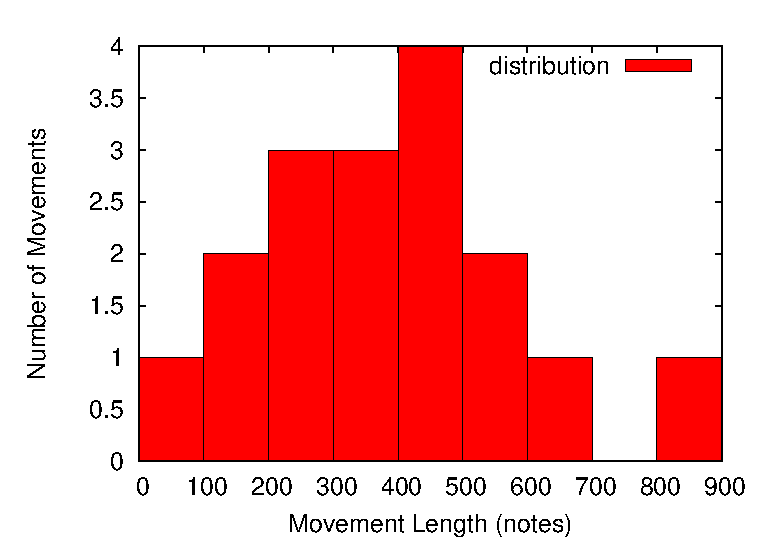
\includegraphics[width=\textwidth]{fig/notes}

   \end{center}
   \caption{Movements Length (in Notes) Distribution}
   \label{fig:notes}
\end{figure*}
\begin{figure*}[tp]
   \begin{center}
      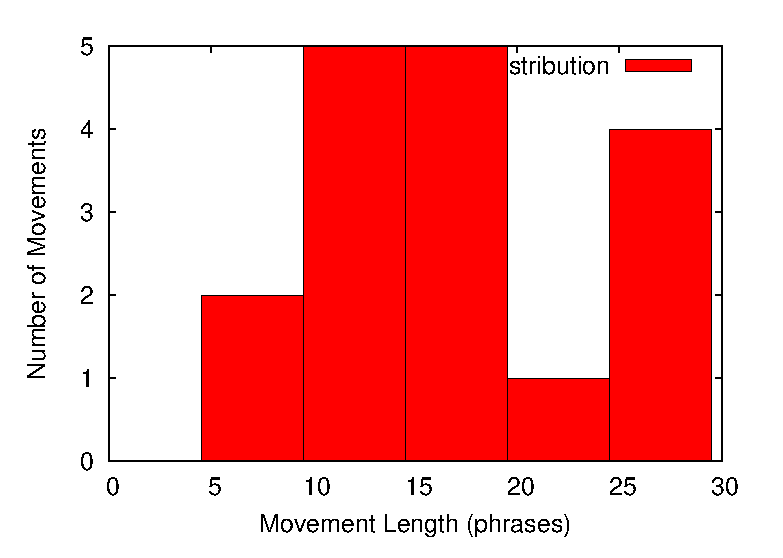
\includegraphics[width=\textwidth]{fig/phrases}

   \end{center}
   \caption{Movements Length (in Phrases) Distribution}
   \label{fig:phrases}
\end{figure*}
\begin{figure*}[tp]
   \begin{center}
      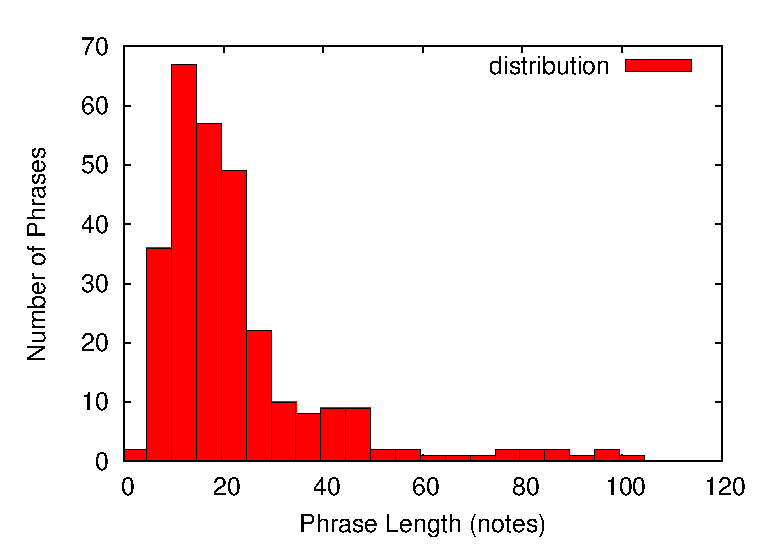
\includegraphics[width=\textwidth]{fig/phrlength}

   \end{center}
   \caption{Phrase Length (in Notes) Distribution}
   \label{fig:phrlength}
\end{figure*}


\begin{table}[bp]
   \centering
   \caption{Performer Music Experience}
   \label{tab:performer}
   \begin{tabular}{lrr}
      \hline
      \textbf{TBD} & \textbf{TBD} & \textbf{TBD}\\
      \hline
      \textbf{TBD} & \textbf{TBD} & \textbf{TBD}\\
      \hline
      \textbf{TBD} & \textbf{TBD} & \textbf{TBD}\\
      \hline
      \textbf{TBD} & \textbf{TBD} & \textbf{TBD}\\
      \hline
      \textbf{TBD} & \textbf{TBD} & \textbf{TBD}\\
      \hline
      \textbf{TBD} & \textbf{TBD} & \textbf{TBD}\\
      \hline
      \textbf{TBD} & \textbf{TBD} & \textbf{TBD}\\
      \hline
      \textbf{TBD} & \textbf{TBD} & \textbf{TBD}\\
      \hline
      \textbf{TBD} & \textbf{TBD} & \textbf{TBD}\\
      \hline
   \end{tabular}
\end{table}
\begin{table}[bp]
   \centering
   \caption{Total Recorded Phrases and Notes Count}
   \label{tab:corpuscount}
   \begin{tabular}{lrrr}
      \hline
      \bf Title&\bf Recordings&\bf Total Phrases&\bf Total Notes\\
      &\bf Count&&\\
      \hline
      No. 1 Mov. I&6&72&1332\\
      No. 1 Mov. II&6&60&882\\
      No. 1 Mov. III&6&102&1566\\
      No. 2 Mov. I&6&108&1920\\
      No. 2 Mov. II&6&36&750\\
      No. 2 Mov. III&6&168&2484\\
      No. 3 Mov. I&6&156&3156\\
      No. 3 Mov. II&6&42&444\\
      No. 3 Mov. III&6&120&2628\\
      No. 4 Mov. I&5&80&2325\\
      No. 4 Mov. II&6&78&1332\\
      No. 4 Mov. III&5&85&1920\\
      No. 5 Mov. I&5&85&3360\\
      No. 5 Mov. II&5&70&1580\\
      No. 5 Mov. III&6&144&3384\\
      No. 6 Mov. I&5&145&4180\\
      No. 6 Mov. II&6&78&2754\\
      \hline
      Total&97&1629&35997\\
      \hline
   \end{tabular}
\end{table}


 %TODO:recording example pic
\framebox{TODO:mention Fig. \ref{fig:exprecording}}
\begin{figure*}[tp]
   \begin{center}
      %TODO:Fig.:Example JSON code
      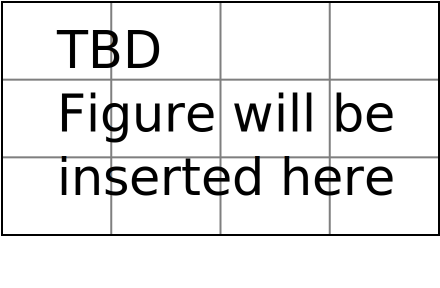
\includegraphics[width=\textwidth]{fig/TBDFigure}

   \end{center}
   \caption{Example Recording Compared to Score (Pianoroll)}
   \label{fig:exprecording}
\end{figure*}

